\documentclass{article}
\usepackage{amsmath}
\usepackage{graphicx}
\usepackage{listings}
\newcommand{\includecode}[2][c]{\lstinputlisting[caption=#2, escapechar=, language=#1]{#2}}
\usepackage{minted}


\begin{document}
\lstset{language=C} 
\title{Homework 5: Feynman problem}
\author{David Jedynak}
\maketitle
\begin{abstract}
 We show how an angled tube can be created in an integer lattice gas method simulation. This angled tube is used with particle sources to perform an experiment to provide insight on the Feynman problem. The momentum transferred from the particles to the tube will be estimated to understand the response of the tube to different densities. The influence of density ratios inside and outside the tube on the force will be observed. The influence of the tube geometry on momentum will also be tested.
\end{abstract}

\section{Introduction}
The Feynman problem presents the question of what will occur when an angled tube attached to a pivot point has fluid pushed out or sucked into the tube. Will the tube rotate clockwise or counter clockwise? My prediction is that the tube will rotate clockwise when air is pushed out of the tube and counter clockwise when air is sucked in, if the experiment is set up as in the figures 1 - 6 below.\newline



The Lattice Gas simulation where this experiment will be executed has constraints that particle momentum and the number of particles must be conserved. The collisions and resulting velocities can be modeled using random processes that can lower the computation cost from prior simulations that would calculate interactions between every particle based on distance, charge, mass, and fields. This can be done because the prior simulations exhibit this random behavior.\newline


\section{Walls}
The Feynman experiment will require 2 Dimensional walls to create a right angled tube. Particles must be reflected if they hit a wall. Particles cannot pass through walls. To accomplish this requirement, velocities in different directions can be swapped. The lattice gas simulation is composed of many cells. Each cell has 9(3 by 3 grid) different values to describe particles motion in a cell.\newline


Here are the indexes for each velocity. The value behind each index is the magnitude of the velocity in that direction\newline
\begin{center}
Indexes ~
\begin{tabular}{l c r}
	\hline
	0 & 1 & 2 \\ \hline
	3 & 4 & 5 \\ \hline
	6 & 7 & 8 \\ 
	\hline
\end{tabular}
\end{center}

\begin{center}
Velocities corresponding to Indexes above ~
\begin{tabular}{l c r}
	\hline
	$(-v_x,+v_y)$ & $(0,+v_y)$ & $(+v_x,+v_y)$ \\ \hline
	$(-v_x,0)$ & $(0,0)$ & $(+v_x,0)$ \\ \hline
	$(-v_x,-v_y)$ & $(0,-v_y)$ & $(+v_x,-v_y)$ \\ 
	\hline
\end{tabular}
\end{center}

\subsection{Walls as Links}
A wall will be composed of links. The links will have an x and y coordinates that will be the same as the lattice cell they are interacting with. Additionally these links will also store the index of the velocity position they will be swapping. Horizontal walls will be switching [0,1,2] will be switched with [8,7,6] respectively. Vertical walls will be switching [0,3,6] will be switched with [8,5,2] respectively. Only one of these sets for each Vertical and Horizontal walls will need to be stored because both will be able to derive the second set's indexes from the first set. 
\vspace{5mm}
Code defining Horizontal Walls:\newline
Note: The horizontal walls link 0, 1, and 2 with 8, 7, and 6 respectively.
\vspace{5mm}
\begin{minted}{c}
//horizontal walls
  for (int x=x0; x<x1+1; x++){
    	links[linkcount][0] = x; //x-position
    	links[linkcount][1] = yy2;
    	links[linkcount][2] = 0;
    	linkcount++;
    	links[linkcount][0] = x; //x-position
    	links[linkcount][1] = yy2;
    	links[linkcount][2] = 1;
    	linkcount++;
    	links[linkcount][0] = x; //x-position 
    	links[linkcount][1] = yy2;
    	links[linkcount][2] = 2;
    	linkcount++;
  }
\end{minted}
\vspace{5mm}
Code Defining Vertical Walls:\newline This wall in particular is also the opening for the tube that can be disabled or enabled.
Note: The vertical walls link 0, 3, and 6 with 8, 5, and 2 respectively.
\vspace{5mm}
\begin{minted}{c}
  //vertical walls
if(close_tube == 1){
  for (int y=yy0; y<yy1+1; y++){
	links[linkcount][0] = x2; //x-position
	links[linkcount][1] = y;
	links[linkcount][2] = 0;
	linkcount++;
	links[linkcount][0] = x2; //x-position
	links[linkcount][1] = y;
	links[linkcount][2] = 3;
	linkcount++;
	links[linkcount][0] = x2; //x-position
	links[linkcount][1] = y;
	links[linkcount][2] = 6;
	linkcount++;
  }
}

\end{minted}
\vspace{5mm}
Additional code added to prevent the tube from leaking particles at several vertices.
\vspace{5mm}
\begin{minted}{c}
//2 links added to prevent leaking on the x0,yy2 and x2,yy0 squares 
	links[linkcount][0] = x0; //x-position
    	links[linkcount][1] = yy2;
    	links[linkcount][2] = 0;
    	linkcount++;
	links[linkcount][0] = x2; //x-position
    	links[linkcount][1] = yy0;
    	links[linkcount][2] = 0;
    	linkcount++;
\end{minted}

Code Defining How particles reflect off of walls (Both horizontal and vertical)
\begin{minted}{c}
void bounceback(){
  tot_vx =0;
  tot_vy =0;
  for (int lc=0; lc<linkcount; lc++){
    //quantity of partices in a given link
    int x=links[lc][0];
    int y=links[lc][1];
    //velocity of the particles in a given link
    int v=links[lc][2];
    int vx=v%3-1;
    int vy=1-v/3;
    int tmp= n[x+vx][y+vy][v];
    //summing all momemtums
    tot_vx += -2*vx*(n[x][y][8-v]-tmp);
    tot_vy += -2*vy*(n[x][y][8-v]-tmp);
    //swapping the particles trying to enter 
    //and leave to have the effect of a wall
    n[x+vx][y+vy][v]= n[x][y][8-v];
    n[x][y][8-v]=tmp;		
  }
  //measure routine stores values for plotting
  Measure();
}
\end{minted}

\section{Calculating Momentum}
 The momentum of the tube can be calculated by relating  the quantity and velocity of the particles being reflected by the tube. The momentum can be described using 2 dimensions x and y. The tube momentum in either direction will be proportional to 2 times the opposite momentum of the difference of the particles attempting to leave or enter the tube/wall. To find the total momentum, the sum of all these particle momentum will be taken over every single "link" or way particles can travel from one lattice cell to another.
 
\vspace{5mm}
$
(\rho_x,\rho_y) = -2*\sum_{link_0}^{link+1} (vel_x*(\Delta particles_x),vel_y*(\Delta particles_y))
 $
\vspace{5mm}

 Accomplishing this in the program requires a calculating in the bounce back routine previously discussed in section 2.1 to iterate through all links and sum this calculation.
 
 \begin{minted}{c}
    int tmp= n[x+vx][y+vy][v];
    //summing all momemtums
    tot_vx += -2*vx*(n[x][y][8-v]-tmp);
    tot_vy += -2*vy*(n[x][y][8-v]-tmp);
\end{minted}
 
\section{Force as a Function of Density Ratios}
As the difference in the source and drain densities increase, the magnitude of the force and momentum should increase. The particles are going to try and find the route of least resistance from source to drain. On this path they will probably collide with the tube and exert force on the tube. This is measured by observing the tube momentum as described in section3. 
\section{Results}
\vspace{5mm}
Note: For figures 1 through 7, the Collisions parameter is set to 100, the source is placed inside the bent tube and the drain is placed at the coordinates (x,y) = (50,50). Both source and drain are the same size.
\vspace{5mm}
\begin{figure}[H]
\centering
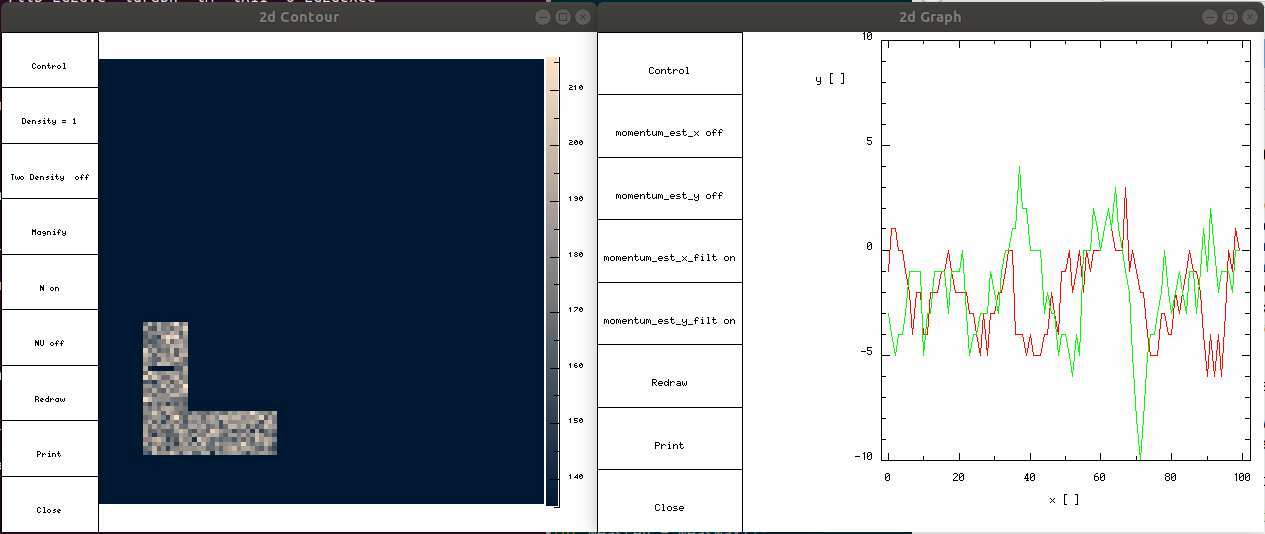
\includegraphics[scale=0.3]{p1_noleakage.png}
\caption{\label{fig} $\rho_x$ is green and $\rho_y$ is red. Image of fully closed tube with source located inside. light color ~ high desity dark color ~low to zero density. The graph to the left shows the averaged x and y momentums centered around 0, so this is a good check that the box is sealed, beacuse otherwise there would be non zero net momentum.}
\end{figure}

\subsection{Influence of source and drain densities on momentum}
\begin{figure}[H]
\centering
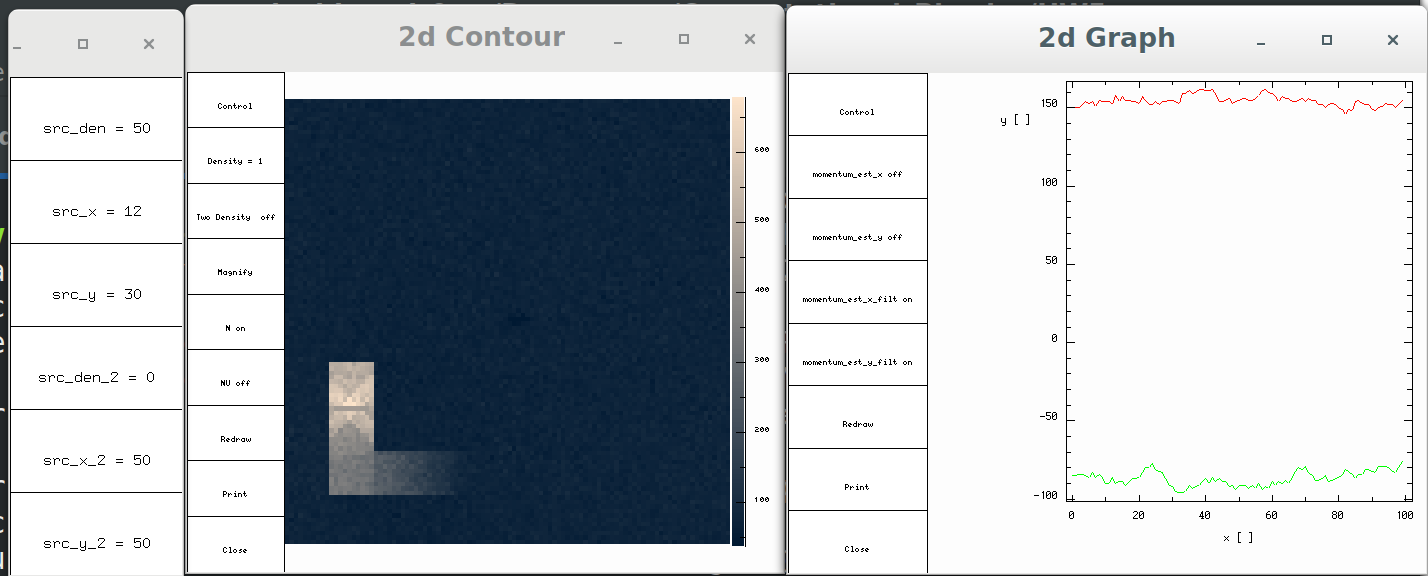
\includegraphics[scale=0.25]{source_50_drain_0.png}
\caption{\label{fig} $\rho_x$ is green and $\rho_y$ is red. Source density is 50 and Drain density is 0. The tube momentum is in the positive y and negative x.}
\end{figure}

\begin{figure}[H]
\centering
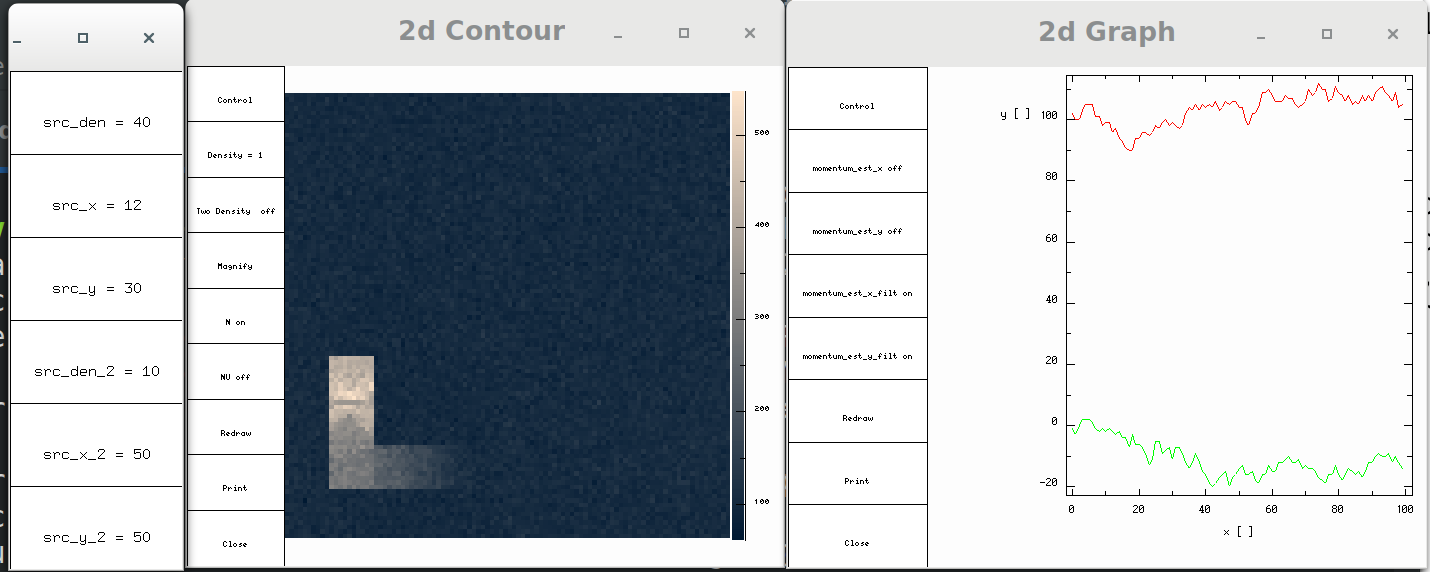
\includegraphics[scale=0.25]{source_40_drain_10.png}
\caption{\label{fig} $\rho_x$ is green and $\rho_y$ is red. Source density is 40 and Drain density is 10.}
\end{figure}

\begin{figure}[H]
\centering
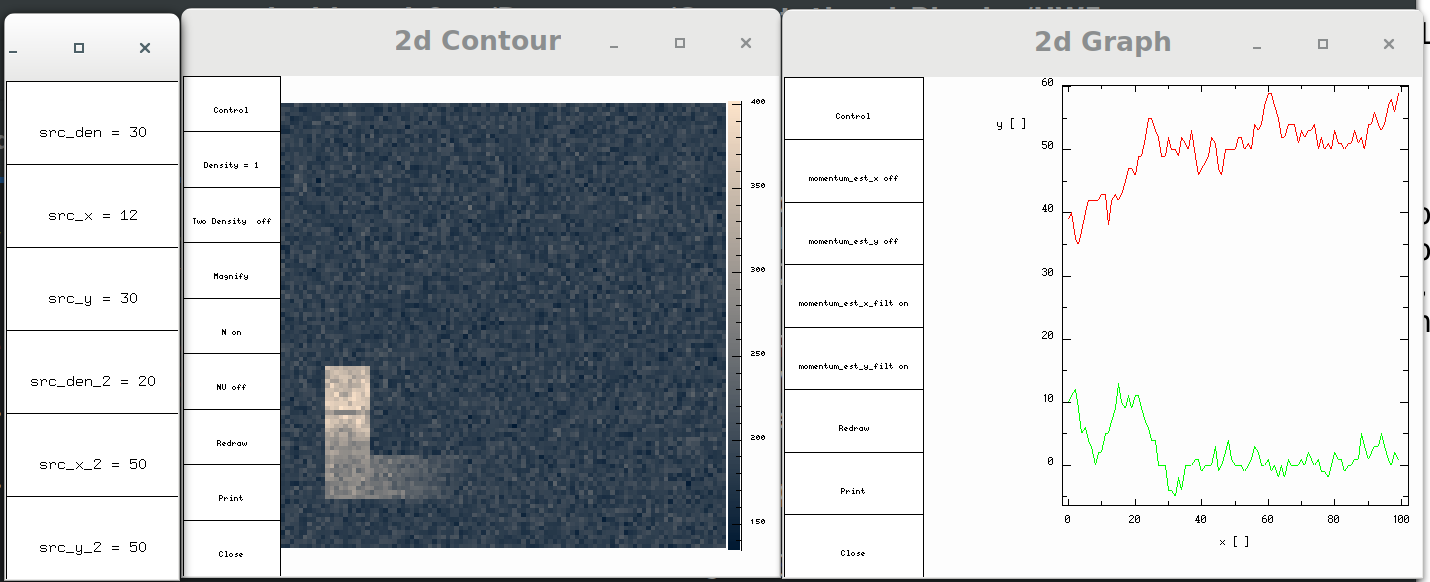
\includegraphics[scale=0.25]{source_30_drain_20.png}
\caption{\label{fig} $\rho_x$ is green and $\rho_y$ is red. Source density is 30 and Drain density is 20.}
\end{figure}

\begin{figure}[H]
\centering
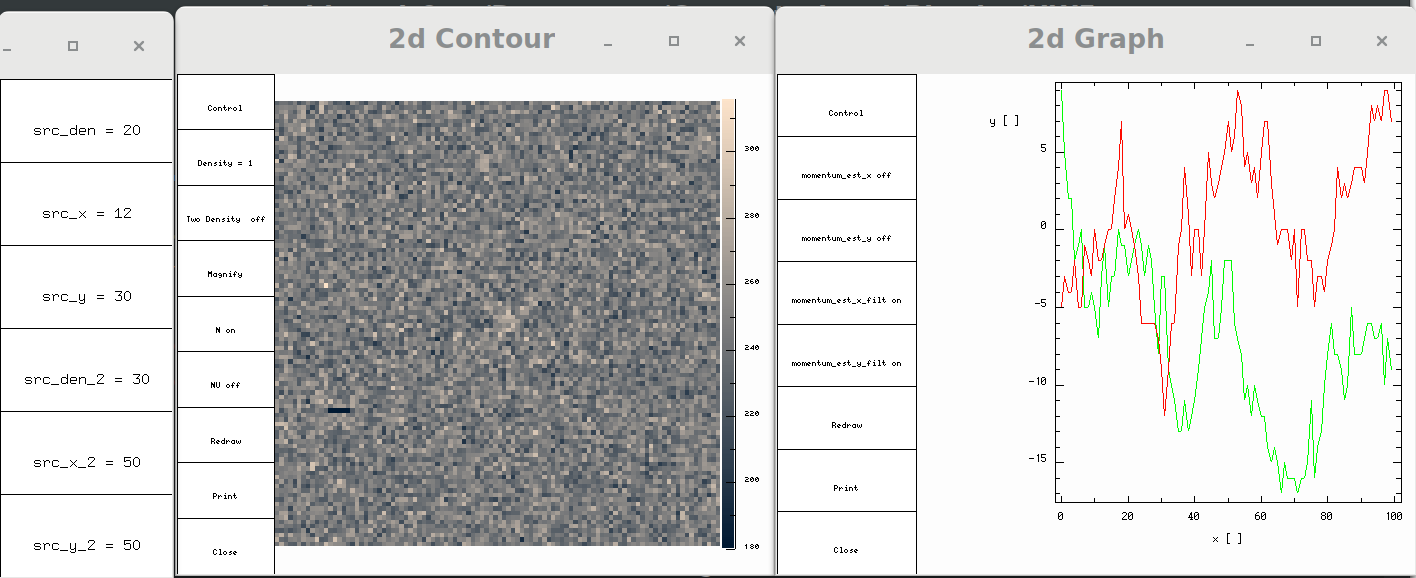
\includegraphics[scale=0.25]{source_20_drain_30.png}
\caption{\label{fig} $\rho_x$ is green and $\rho_y$ is red. Source density is 20 and Drain density is 30.}
\end{figure}

\begin{figure}[H]
\centering
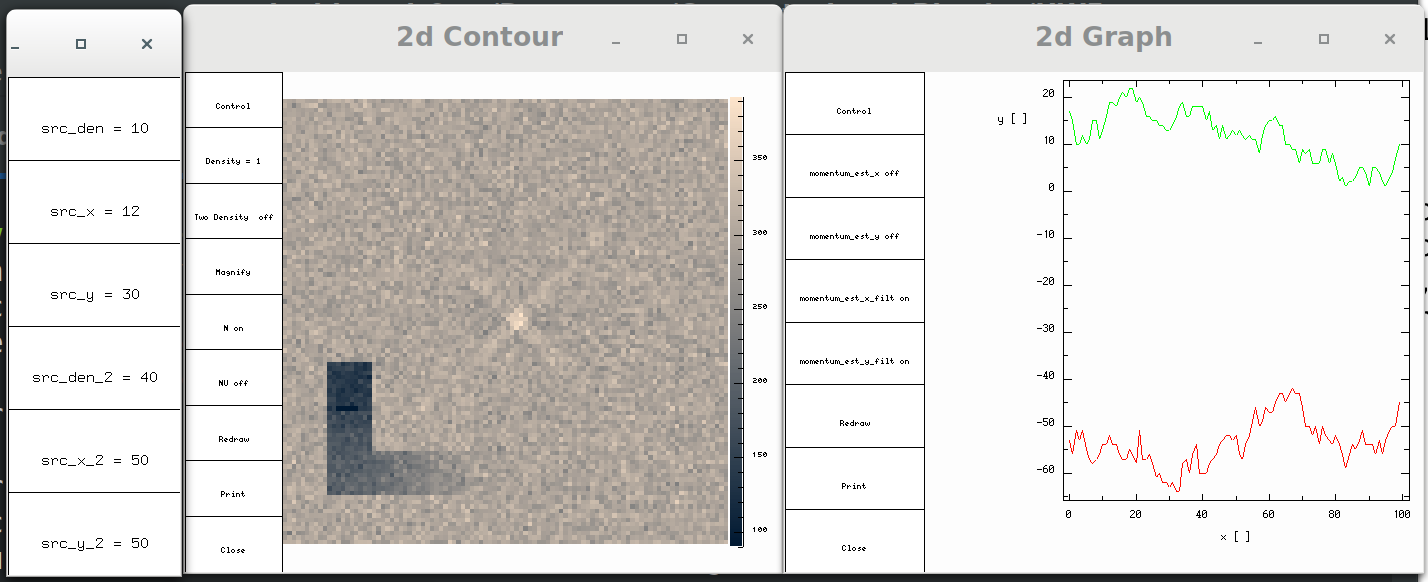
\includegraphics[scale=0.25]{source_10_drain_40.png}
\caption{\label{fig} $\rho_x$ is green and $\rho_y$ is red. Source density is 10 and Drain density is 50.}
\end{figure}

\begin{figure}[H]
\centering
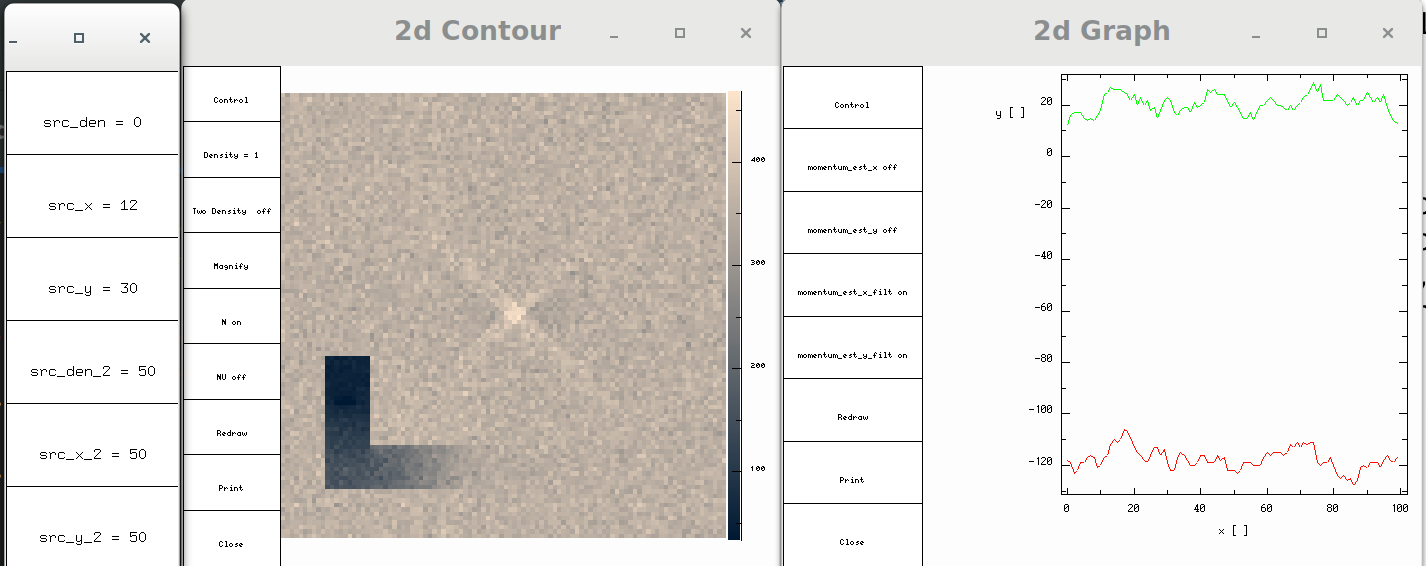
\includegraphics[scale=0.25]{source_0_drain_50.png}
\caption{\label{fig} $\rho_x$ is green and $\rho_y$ is red. Source density is 0 and Drain density is 50. The tube momentum is in the negative y and positive x.}
\end{figure}

\vspace{5mm}
\subsection{Force as a function of density ratios}
Observing changes in momentum due to changing outlet dimensions. Collisions are set to 100. the source is set to 15 and the drain is set to 0.
\vspace{5mm}

\begin{figure}[H]
\centering
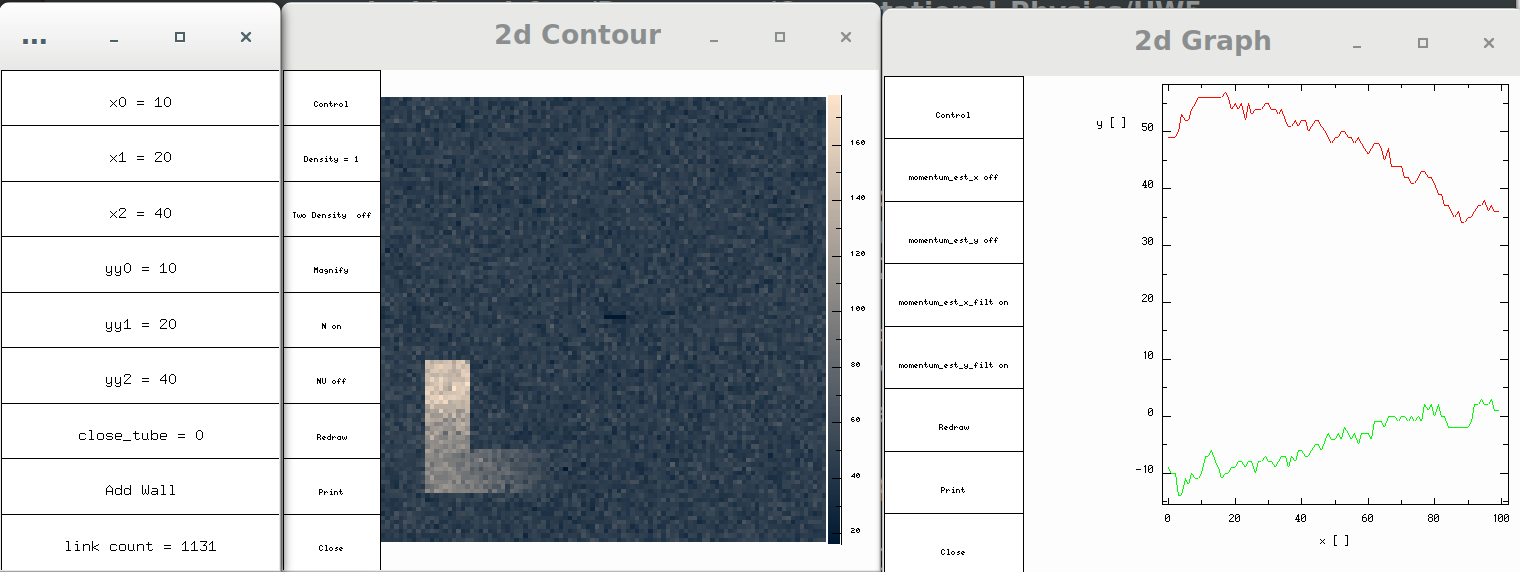
\includegraphics[scale=0.25]{df_10.png}
\caption{\label{fig} $\rho_x$ is green and $\rho_y$ is red. Outline size is 10}
\end{figure}

\begin{figure}[H]
\centering
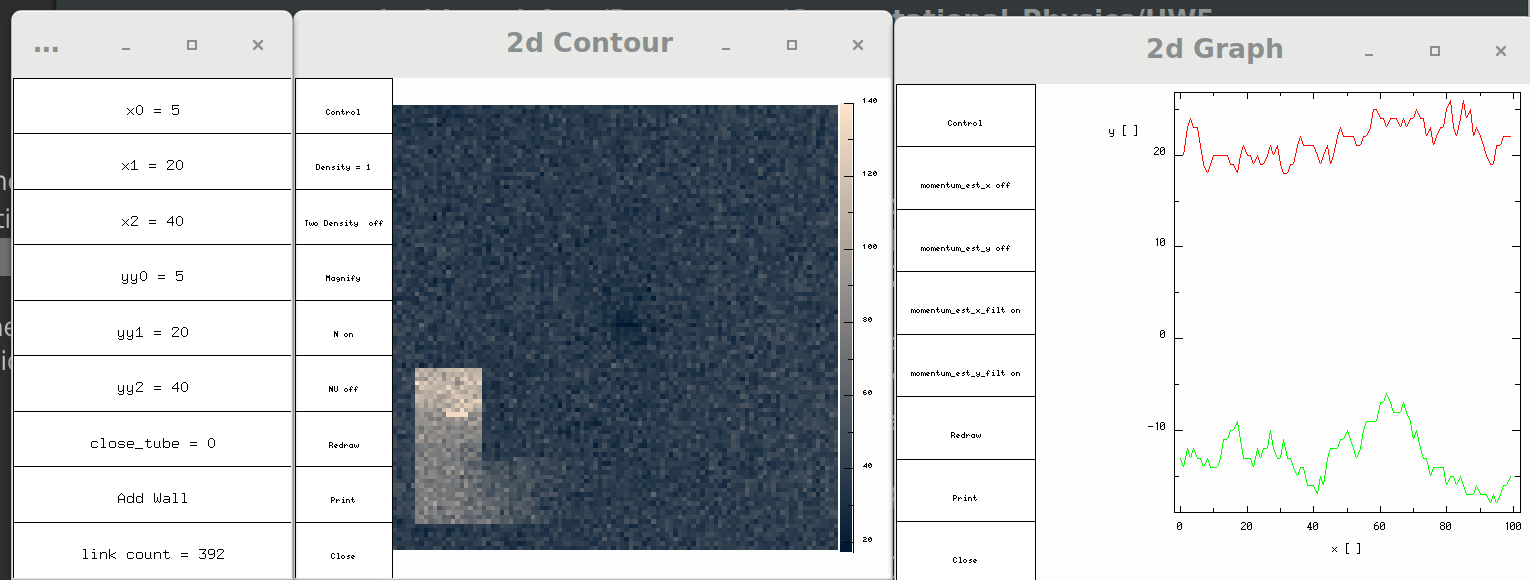
\includegraphics[scale=0.25]{df_15.png}
\caption{\label{fig} $\rho_x$ is green and $\rho_y$ is red. Outlet size is 15.}
\end{figure}

\begin{figure}[H]
\centering
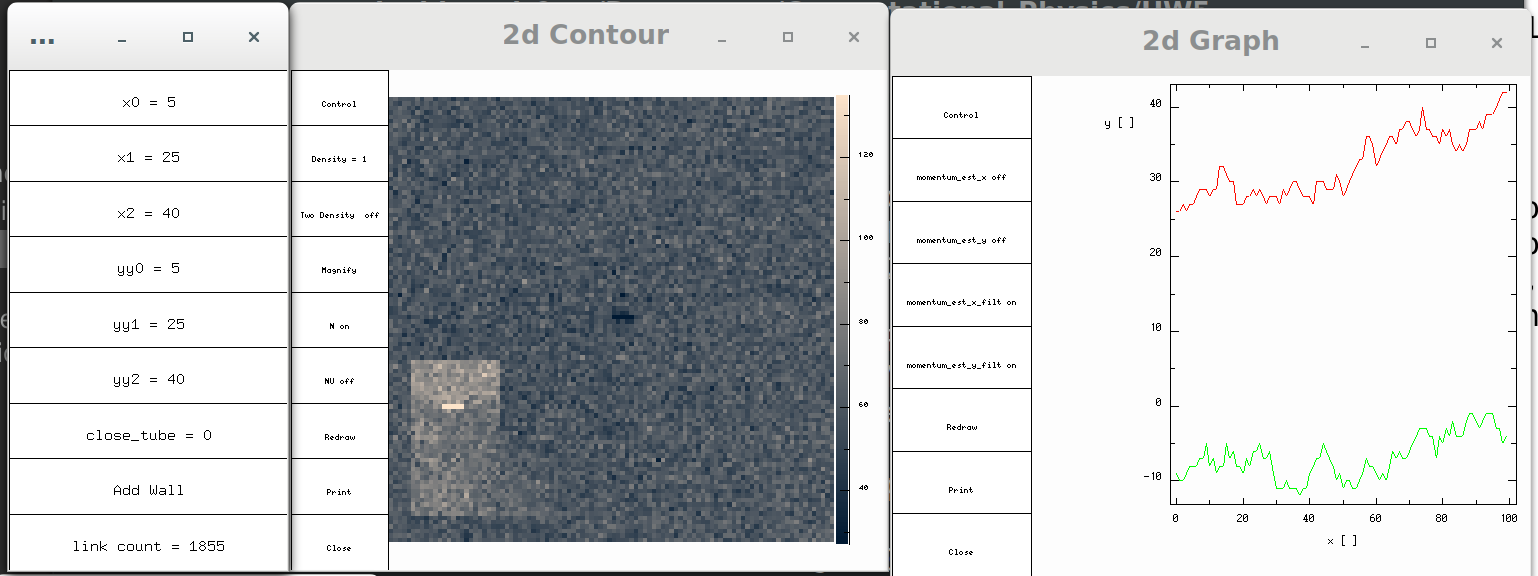
\includegraphics[scale=0.25]{df_20.png}
\caption{\label{fig} $\rho_x$ is green and $\rho_y$ is red. Outlet size is 20.}
\end{figure}



\section{Conclusions}
Figure 1 shows a tube fully sealed with no leaking, this is an important step because if there were leaks in the tube, this would cause error in the Feynman experiment momentum measurements.\newline
By observing the figures 2 through 7, it can be seen that as the source and drain densities switch, the resulting momentum change for x and y do not appear to be equivalent. One notable change is that when source=50 and drain=0 the y momentum was around 150 and the y momentum was around -90. When the source=0 and the drain=50, the y momentum was around -120 and the x momentum was around 20. Additionally, in figure 3 and 4 where source and drain switch from being 30 and 20 to 20 and 30, they are extremely different in appearance. Perhaps this test required more time to reach steady state, but this was also observed using source and drain densities of 3 and 2 to 2 and 3.\newline
As the outlet size increased, the momentum in both x and y dimensions decreased. This can be observed in figures 8 through 10. Y momentum changes from 50 to 20, X did not change very much -20 to -10. This hypothesized characteristic might be due to noise and potentially invalid. Figure 10 shows the y going back up to 40.
Running the simulation will low source densities around 0 to 5 yielded very noisy data. The data from the 0 to 50 source densities yielded much more distinct changes in x and y momentum.


\appendix
\section{Code}
\lstinputlisting[language=C]{/home/david/Documents/Computational_Physics/HW5/LG2d.c}
\end{document}
  
